\documentclass[11pt,a4paper]{article}

% ---------------------------------------------------------------------------
% Paquets
% ---------------------------------------------------------------------------
\usepackage[utf8]{inputenc}
\usepackage[T1]{fontenc}
\usepackage[french]{babel}
\usepackage{lmodern}
\usepackage[margin=2.3cm]{geometry}
\usepackage{amsmath,amssymb}
\usepackage{booktabs}
\usepackage{longtable}
\usepackage{tabularx}
\usepackage{array}
\usepackage{graphicx}
\usepackage{float}
\usepackage[hidelinks]{hyperref}
\usepackage{enumitem}

\graphicspath{{../figures/}}
\newcolumntype{Y}{>{\raggedright\arraybackslash}X}

\title{Calibrage d'une courbe de swap SOFR\\et pricing d'un cap 5 ans à 3\,\%}
\author{Olivier TAGALI}
\date{3 novembre 2026}

\begin{document}
\maketitle

% ---------------------------------------------------------------------------
\section{Résumé exécutif}
% ---------------------------------------------------------------------------
Le cap SOFR 5 ans trimestriel à 3\,\% sur 10\,M\$ vaut \textbf{223\,799\,\$}, soit 2,24\,\% du notionnel, avec une volatilité de Black de 20\,\%.

\begin{table}[H]
\centering
\begin{tabular}{lr}
\toprule
Indicateur & Valeur \\
\midrule
Prix du cap (19 caplets) & 223\,799\,\$ \\
Prix du floor 5 ans à 3\,\% & 214\,377\,\$ \\
Erreur max de re-pricing des swaps & 1,2e-12 pb \\
Vega (+1 point de vol) & 6\,572\,\$ \\
DV01 (+1 pb parallèle) & 2\,087\,\$ \\
Choc +100 pb / $-$100 pb & +270\,593\,\$ / $-$152\,602\,\$ \\
Temps de calcul & $<$ 10 ms (0,5 s avec graphiques) \\
\bottomrule
\end{tabular}
\end{table}

La courbe est calibrée exactement sur les swaps. La parité cap-floor tient à 6e-11\,\$ près, ce qui valide la chaîne courbe $\rightarrow$ forwards $\rightarrow$ Black.

% ---------------------------------------------------------------------------
\section{Contexte et objectif}
% ---------------------------------------------------------------------------
Un client a emprunté à taux variable SOFR et veut plafonner son coût de financement à 3\,\% sur 5 ans. Le desk lui vend un cap : chaque trimestre, si le SOFR dépasse 3\,\%, le cap paie la différence sur 10\,M\$.

Pour fixer ce prix, il faut deux briques : une courbe SOFR calibrée sur le marché (pour les forwards et l'actualisation), puis un modèle d'option sur chaque taux forward (Black). Le modèle Black-Scholes sur un sous-jacent action ne convient pas : le sous-jacent est un taux forward différent pour chaque période, et il doit être lu sur la courbe.

% ---------------------------------------------------------------------------
\section{Données et conventions}
% ---------------------------------------------------------------------------
Les données sont synthétiques, issues de l'énoncé. La date de valorisation est fixée au 3 novembre 2026.

\begin{table}[H]
\centering
\begin{tabularx}{\textwidth}{lY}
\toprule
Paramètre & Valeur \\
\midrule
Swaps SOFR cotés & 1 an : 2,00\,\% $\cdot$ 3 ans : 2,50\,\% $\cdot$ 5 ans : 3,00\,\% \\
Swaps interpolés & 2 ans : 2,25\,\% $\cdot$ 4 ans : 2,75\,\% (linéaire sur les taux de swap) \\
Jambe fixe des swaps & Annuelle \\
Cap & $N = 10$\,M\$, $K = 3\,\%$, 5 ans, trimestriel (20 périodes) \\
Volatilité & $\sigma$ de Black $= 20\,\%$ (lognormale, plate) \\
Base de calcul & Act/360 pour les accruals et l'axe des temps \\
Taux zéro & Capitalisation continue, $P(0,t) = \exp(-r(t)\,t)$ \\
\bottomrule
\end{tabularx}
\end{table}

Trois choix méritent d'être assumés explicitement. Le premier caplet est fixé aujourd'hui : il n'a pas d'optionalité et sort du prix (sa valeur intrinsèque est nulle car le forward est à 1,99\,\%). Les dates ne sont pas ajustées en jours ouvrés. Le forward simple sur la période sert de proxy au SOFR composé dans la période.

% ---------------------------------------------------------------------------
\section{Méthodologie}
% ---------------------------------------------------------------------------
La chaîne de calcul suit quatre étapes : bootstrap, interpolation, forwards, Black.

\paragraph{1. Bootstrap.} Un swap au pair vaut zéro, donc sa jambe fixe plus le remboursement fictif du notionnel vaut 1 :
\begin{equation}
1 = s(T_n) \sum_{i=1}^{n} \tau_i P(0,t_i) + P(0,T_n)
\end{equation}
Avec un coupon par an et un pilier par an, chaque maturité n'ajoute qu'une inconnue. On l'isole directement, sans solveur :
\begin{equation}
P(0,T_n) = \frac{1 - s_n \sum_{i<n} \tau_i P(0,t_i)}{1 + s_n \tau_n}, \qquad r(T_n) = -\frac{\ln P(0,T_n)}{T_n}
\end{equation}

\paragraph{2. Interpolation.} Entre les piliers, les taux zéro sont interpolés par spline cubique naturelle, pour une courbe lisse. L'interpolation linéaire est gardée comme contrôle. Avant 1 an, extrapolation plate (aucune donnée court terme).

\paragraph{3. Forwards trimestriels.} Le taux forward simple entre deux dates de fixing se lit sur la courbe :
\begin{equation}
L(t_{i-1},t_i) = \frac{1}{\tau_i}\left(\frac{P(0,t_{i-1})}{P(0,t_i)} - 1\right)
\end{equation}

\paragraph{4. Formule de Black.} Chaque caplet est un call sur le forward, payé en $t_i$, avec une variance accumulée jusqu'au fixing $t_{i-1}$ :
\begin{equation}
C_i = N \tau_i P(0,t_i)\,[F_i N(d_1) - K N(d_2)], \quad d_{1,2} = \frac{\ln(F_i/K) \pm \tfrac12 \sigma^2 t_{i-1}}{\sigma\sqrt{t_{i-1}}}
\end{equation}

Le prix du cap est la somme des caplets 2 à 20. Le floor utilise la même formule côté put.

% ---------------------------------------------------------------------------
\section{Résultats}
% ---------------------------------------------------------------------------
La courbe calibrée remonte de 1,98\,\% à 2,99\,\% (zéro continu) entre 1 et 5 ans, et les forwards 3M passent au-dessus du strike de 3\,\% à partir de 2,5 ans environ.

\subsection{Courbe bootstrappée}

\begin{table}[H]
\centering
\begin{tabular}{lrrrrr}
\toprule
Maturité & Swap & $t$ (Act/360) & $P(0,T)$ & $r(T)$ continu & Écart de re-pricing \\
\midrule
1 an    & 2,000\,\% & 1,0139 & 0,980125 & 1,9800\,\% & 1,2e-12 pb \\
2 ans*  & 2,250\,\% & 2,0306 & 0,955777 & 2,2275\,\% & 3,1e-13 pb \\
3 ans   & 2,500\,\% & 3,0444 & 0,927358 & 2,4772\,\% & 1,7e-13 pb \\
4 ans*  & 2,750\,\% & 4,0583 & 0,895136 & 2,7297\,\% & 3,5e-14 pb \\
5 ans   & 3,000\,\% & 5,0722 & 0,859461 & 2,9859\,\% & 1,4e-13 pb \\
\bottomrule
\end{tabular}
\end{table}

* Maturités interpolées. Le re-pricing des swaps sur la courbe retrouve chaque cotation à la précision machine : le calibrage est exact par construction.

\begin{figure}[H]
\centering
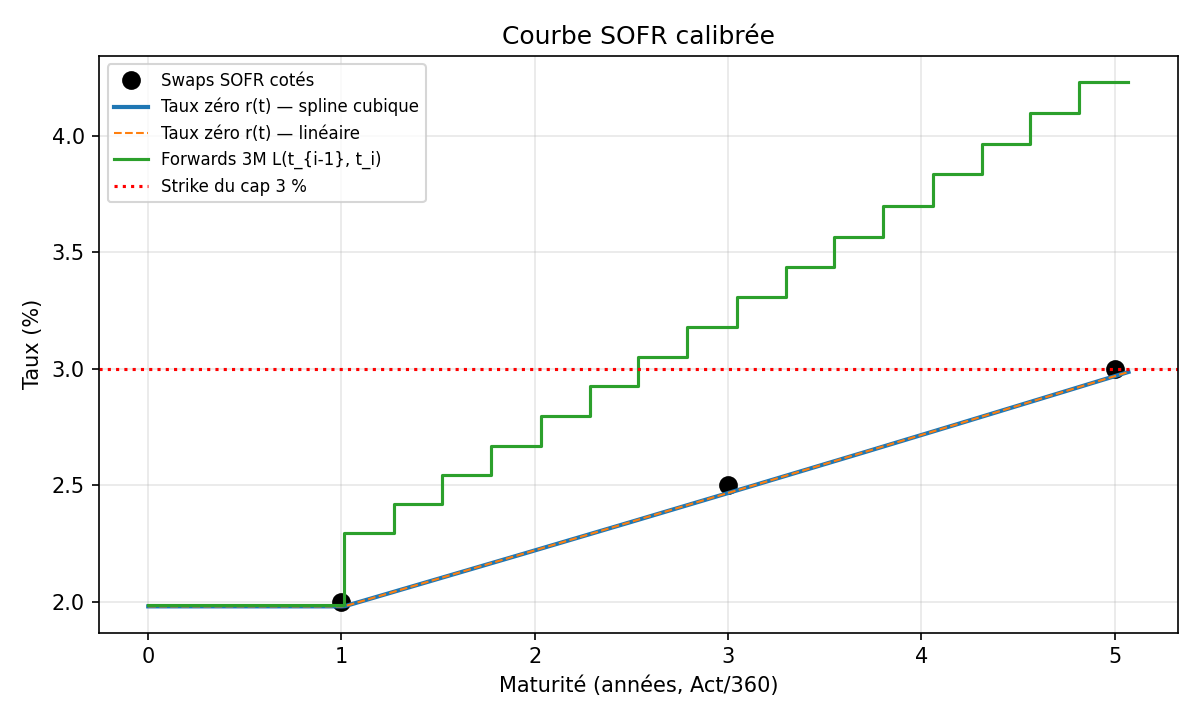
\includegraphics[width=0.9\textwidth]{1_courbe_calibree.png}
\caption{Courbe SOFR calibrée : swaps cotés, taux zéro et forwards 3M}
\end{figure}

Les taux zéro sont légèrement sous les taux de swap, ce qui est normal sur une courbe croissante. Spline et interpolation linéaire sont presque confondues ; la différence de prix du cap est de 33\,\$ (223\,766\,\$ en linéaire).

\subsection{Caplets et prix du cap}

\begin{longtable}{rlrrrr}
\toprule
\# & Paiement & Fixing $t$ & Forward 3M & $P(0,t)$ & Valeur (\$) \\
\midrule
\endhead
1  & 03/02/2027 & 0,000 & 1,985\,\% & 0,99495 & exclu (intrinsèque 0) \\
2  & 03/05/2027 & 0,256 & 1,985\,\% & 0,99009 & 0 \\
3  & 03/08/2027 & 0,503 & 1,985\,\% & 0,98510 & 5 \\
4  & 03/11/2027 & 0,758 & 1,985\,\% & 0,98013 & 31 \\
5  & 03/02/2028 & 1,014 & 2,295\,\% & 0,97441 & 560 \\
6  & 03/05/2028 & 1,269 & 2,419\,\% & 0,96855 & 1\,326 \\
7  & 03/08/2028 & 1,519 & 2,543\,\% & 0,96230 & 2\,507 \\
8  & 03/11/2028 & 1,775 & 2,670\,\% & 0,95578 & 3\,996 \\
9  & 03/02/2029 & 2,031 & 2,798\,\% & 0,94899 & 5\,751 \\
10 & 03/05/2029 & 2,286 & 2,924\,\% & 0,94218 & 7\,433 \\
11 & 03/08/2029 & 2,533 & 3,051\,\% & 0,93489 & 9\,759 \\
12 & 03/11/2029 & 2,789 & 3,180\,\% & 0,92736 & 11\,987 \\
13 & 03/02/2030 & 3,044 & 3,309\,\% & 0,91958 & 14\,298 \\
14 & 03/05/2030 & 3,300 & 3,437\,\% & 0,91183 & 16\,094 \\
15 & 03/08/2030 & 3,547 & 3,567\,\% & 0,90360 & 19\,024 \\
16 & 03/11/2030 & 3,803 & 3,700\,\% & 0,89514 & 21\,491 \\
17 & 03/02/2031 & 4,058 & 3,834\,\% & 0,88645 & 23\,980 \\
18 & 03/05/2031 & 4,314 & 3,965\,\% & 0,87785 & 25\,550 \\
19 & 03/08/2031 & 4,561 & 4,097\,\% & 0,86875 & 28\,812 \\
20 & 03/11/2031 & 4,817 & 4,229\,\% & 0,85946 & 31\,198 \\
\midrule
\multicolumn{5}{l}{\textbf{Total}} & \textbf{223\,799} \\
\bottomrule
\end{longtable}

La valeur est concentrée en fin de vie : les cinq derniers caplets pèsent 58\,\% du prix. Ils combinent forwards dans la monnaie (3,7\,\% à 4,2\,\%) et plus de temps pour la volatilité. Les caplets de la première année valent presque zéro, car le forward y est à 1,99\,\%, loin sous le strike.

% ---------------------------------------------------------------------------
\section{Analyse de sensibilité}
% ---------------------------------------------------------------------------
Le cap est long vega (+6\,572\,\$ par point de vol) et long taux (+2\,087\,\$ par pb), avec une forte convexité aux chocs de taux.

\subsection{Volatilité}

\begin{figure}[H]
\centering
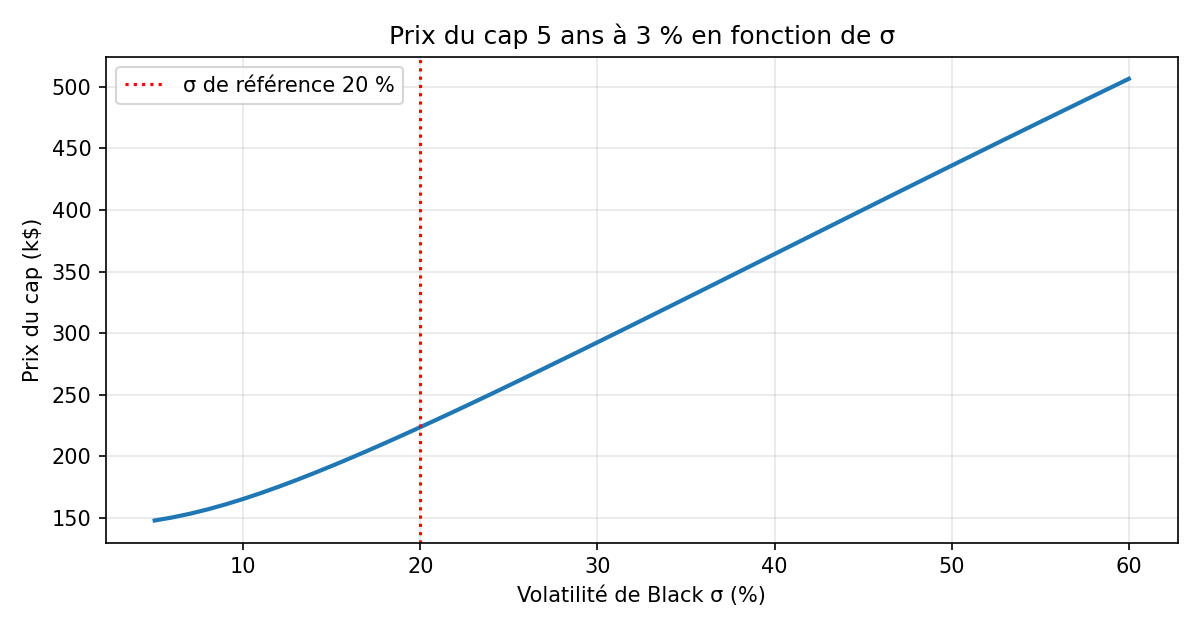
\includegraphics[width=0.85\textwidth]{3_cap_vs_sigma.png}
\caption{Prix du cap en fonction de $\sigma$}
\end{figure}

Le prix passe de 165\,557\,\$ à $\sigma = 10\,\%$ à 364\,223\,\$ à $\sigma = 40\,\%$. La relation est presque linéaire autour de 20\,\%, car le cap est proche de la monnaie en moyenne. C'est le sens de l'avertissement de l'énoncé : une erreur de 2 points sur la vol décale le prix d'environ 13\,000\,\$, soit 6\,\%.

\subsection{Taux}

\begin{figure}[H]
\centering
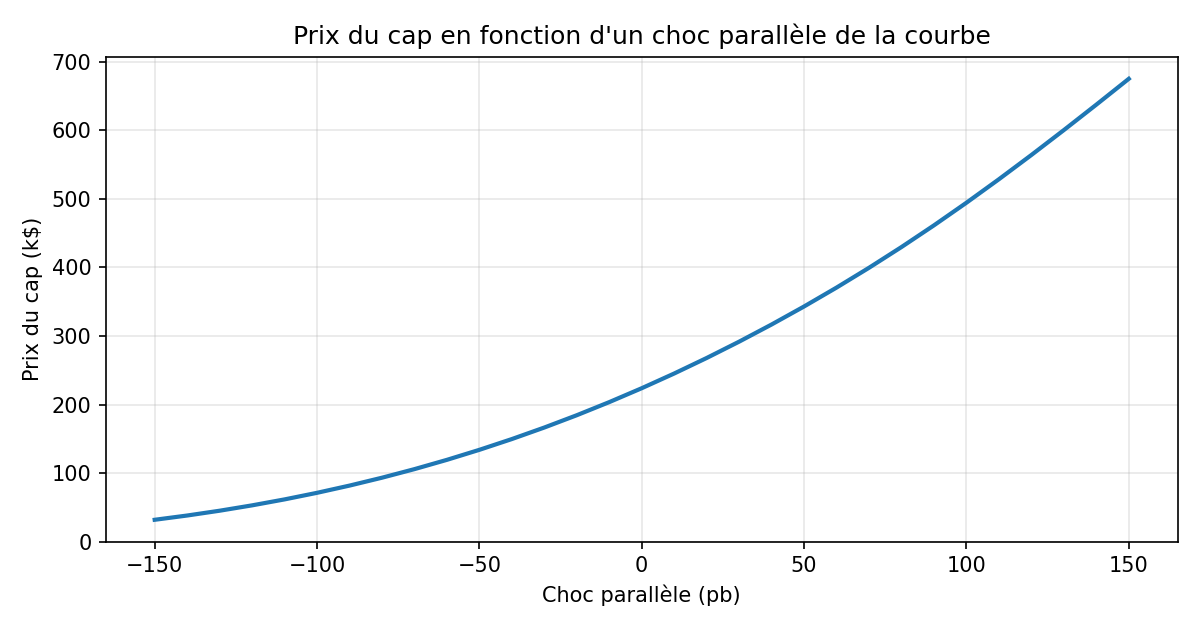
\includegraphics[width=0.85\textwidth]{4_cap_vs_taux.png}
\caption{Prix du cap en fonction d'un choc parallèle de la courbe}
\end{figure}

Un choc +100 pb ajoute 270\,593\,\$, un choc $-$100 pb retire seulement 152\,602\,\$. Cette asymétrie est la convexité (gamma) d'une option : la perte est bornée par la prime, le gain ne l'est pas.

\begin{table}[H]
\centering
\begin{tabular}{lr}
\toprule
Cotation choquée de +1 pb & Variation du cap (\$) \\
\midrule
Swap 1 an & $-$571 \\
Swap 3 ans & $-$980 \\
Swap 5 ans & +3\,631 \\
Somme ($\approx$ DV01 parallèle) & +2\,080 \\
\bottomrule
\end{tabular}
\end{table}

Les deltas négatifs sur 1 et 3 ans surprennent au premier abord. Monter le swap 3 ans à 5 ans inchangé relève les forwards avant 3 ans mais abaisse ceux entre 3 et 5 ans, où se trouve l'essentiel de la valeur. Le risque du cap est donc porté par le pilier 5 ans : c'est là que le desk se couvre.

\subsection{Parité cap-floor}

Le floor 5 ans à 3\,\% vaut 214\,377\,\$. La différence cap $-$ floor (9\,421,32\,\$) égale la valeur du swap payeur forward à 3\,\% à 6e-11\,\$ près. Ce contrôle ne dépend pas du modèle de vol : il valide la cohérence entre forwards et actualisation.

% ---------------------------------------------------------------------------
\section{Cas particuliers et robustesse}
% ---------------------------------------------------------------------------
Avec des swaps plats à 3\,\%, le bootstrap renvoie bien une courbe zéro plate à 2,955\,\%, et des forwards 3M constants à 2,966\,\%.

Les zéros sont sous 3\,\% car 3\,\% en annuel Act/360 correspond à 2,955\,\% en continu. Les forwards 3M (2,966\,\%) sont aussi sous 3\,\% : un taux trimestriel équivalent est plus bas qu'un taux annuel. Le cap est donc légèrement hors de la monnaie : il vaut 150\,037\,\$ contre 164\,973\,\$ pour le floor. Le résultat est cohérent, mais rappelle qu'un strike « égal au taux de swap » n'est pas exactement à la monnaie.

Côté robustesse, la courbe est lisse entre 1 et 5 ans, sans oscillation de la spline. Le calcul complet tourne en moins de 10 ms et 0,5 s avec les graphiques, loin sous la cible de 3 s.

% ---------------------------------------------------------------------------
\section{Limites, pistes d'amélioration et points d'entretien}
% ---------------------------------------------------------------------------
La principale limite est la volatilité plate à 20\,\% : en pratique, chaque caplet a sa propre vol, lue sur une surface de marché.

\begin{table}[H]
\centering
\small
\begin{tabularx}{\textwidth}{>{\raggedright\arraybackslash}p{3.2cm}YY}
\toprule
Limite & Effet & Amélioration \\
\midrule
Vol plate unique & Sous-évalue ou surévalue certains caplets (smile, structure par terme) & Stripping des vols caplets depuis les vols de cap cotées, puis SABR par maturité \\
Pas de données avant 1 an & Forwards plats à 1,99\,\% la première année & Ajouter fixings SOFR, futures SOFR 1M/3M \\
Seulement 3 swaps & Courbe dépendante de l'interpolation des taux de swap & Plus de piliers (2, 4, 7, 10 ans), interpolation monotone convexe \\
Forward simple comme proxy & Ignore la composition quotidienne du SOFR (taux backward-looking) & Modèle de caplet sur taux composé (Lyashenko-Mercurio) \\
Black lognormal & Inutilisable si les taux deviennent négatifs ou très bas & Black décalé (shifted) ou Bachelier (vol normale) \\
Dates non ajustées & Écarts de quelques jours sur les accruals & Calendrier US, convention Modified Following \\
\bottomrule
\end{tabularx}
\end{table}

Points à défendre en entretien :
\begin{itemize}[nosep]
  \item Pourquoi la variance s'arrête au fixing $t_{i-1}$ et l'actualisation va jusqu'au paiement $t_i$.
  \item Pourquoi le premier caplet est exclu, et pourquoi un strike égal au taux de swap n'est pas ATM.
  \item Pourquoi la parité cap-floor est le meilleur test de cohérence courbe-pricer.
  \item Pourquoi les deltas aux piliers 1 et 3 ans sont négatifs, et où se couvrir.
  \item Ce que change le passage de LIBOR (forward-looking) au SOFR (backward-looking composé).
\end{itemize}

% ---------------------------------------------------------------------------
\appendix
\section{Annexe : structure du code et exécution}
% ---------------------------------------------------------------------------
Le code tient dans un fichier, \texttt{sofr\_cap\_pricing.py} ; il se lance avec \texttt{python sofr\_cap\_pricing.py} et écrit les graphiques dans \texttt{./figures}. Dépendances : numpy, scipy, matplotlib, python-dateutil.

\begin{table}[H]
\centering
\small
\begin{tabularx}{\textwidth}{>{\raggedright\arraybackslash}p{5.6cm}Y}
\toprule
Fonction & Rôle \\
\midrule
\texttt{bootstrap\_swap\_curve(T, swap\_rates)} & Interpole les swaps à 2 et 4 ans, bootstrappe $P(0,T)$ et $r(T)$, renvoie un objet \texttt{ZeroCurve} \\
\texttt{ZeroCurve.r / df / forward} & Taux zéro interpolé, facteur d'actualisation, forward simple entre deux dates \\
\texttt{swap\_par\_rate(curve, years)} & Recalcule le taux de swap au pair : test d'ajustement \\
\texttt{black\_caplet(...)} & Formule de Black pour un caplet ou un floorlet \\
\texttt{caplet\_table(curve, ...)} & Échéancier trimestriel, forwards, valeurs de chaque caplet \\
\texttt{cap\_price(N, K, curve, sigma)} & Prix du cap (ou du floor) = somme des caplets 2 à 20 \\
\texttt{sensitivities(curve, price)} & Vega, DV01, chocs $\pm$100 pb, deltas par pilier (re-bootstrap) \\
\texttt{cap\_floor\_parity(curve, table)} & Contrôle cap $-$ floor = swap payeur forward \\
\texttt{make\_figures(...)} & Les quatre graphiques (courbe, caplets, prix vs $\sigma$, prix vs taux) \\
\bottomrule
\end{tabularx}
\end{table}

Les paramètres (date, swaps, $N$, $K$, $\sigma$) sont en tête de fichier : on peut relancer le projet sur d'autres cotations en changeant ces lignes.

\end{document}
